\documentclass[10pt,a4paper]{article}

\usepackage[utf8x]{inputenc}
\usepackage[T1]{fontenc}

%\usepackage{stringenc} % for grffile
\usepackage{ucs}%utf8x and UCS are obsolete, but it still works, so don't fix it
\usepackage{amsthm} %numéroter les questions
\usepackage[english]{babel}
\usepackage{datetime}
\usepackage{scrextend} %\footref{}
%\usepackage{xspace} % typographie IN
\usepackage{hyperref}% hyperliens
\usepackage{listings}
\usepackage[all]{hypcap} %lien pointe en haut des figures
\usepackage[english]{varioref} %voir x p y
\usepackage{fancyhdr}% en têtes
%\input cyracc.def
\usepackage[]{graphicx} %include pictures
%\usepackage[encoding,inputencoding=utf8,filenameencoding=utf8]{grffile}
%\usepackage[extendedchars,inputencoding=latin1,filenameencoding=latin1]{grffile}
%\usepackage[siunitx ]{circuitikz}
%\usepackage{gnuplottex}
\usepackage{ifthen}
\graphicspath{{./figures/}}
\usepackage{array}
\usepackage{amsmath}
\usepackage[]{xcolor}
\usepackage{tikz}
\usepackage{tikz-timing}
\usetikzlibrary{babel}
\usetikzlibrary{scopes}
\usetikzlibrary{backgrounds}

\usepackage{enumitem}
\usepackage[top=1 in, bottom=1 in, left=1.3 in, right=1 in]{geometry} % Yeah, that's bad to play with margins
\usepackage[]{pdfpages}
\usepackage{pdflscape}
\usepackage[]{attachfile}

\usepackage{booktabs}
\usepackage{rotating}

\newcommand{\version}{v1.0.1}

%cyr
%\newcommand\textcyr[1]{{\fontencoding{OT2}\fontfamily{wncyr}\selectfont #1}}


\newboolean{corrige}
%\setboolean{corrige}{true}%corrigé
\setboolean{corrige}{false}% pas de corrigé

%\newboolean{annexes}
%\setboolean{annexes}{true}%annexes
%\setboolean{annexes}{false}% pas de annexes

%\newboolean{mos}
%\setboolean{mos}{true}%annexes
%\setboolean{mos}{false}% pas de annexes

%\usepackage{aeguill} %guillemets

%% fancy header & foot
\pagestyle{fancy}
\lhead{[ELEC-H-473] Microprocessor Architectures: RiSC16 1--2/4}
\rhead{\version\\ page \thepage}
\chead{\ifthenelse{\boolean{corrige}}{Corrigé}{}}
\cfoot{}
%%

\pdfinfo{
/Author (Yannick Allard, ULB -- BEAMS)
/Title (Labo 1 ELEC-H-473, RiSC16_1-2/4)
/ModDate (D:\pdfdate)
}

\hypersetup{
pdftitle={Lab 1 [ELEC-H-473] Microprocessor Architectures},
pdfauthor={Yannick Allard, ©2013-2016 ULB - BEAMS  },
pdfsubject={RiSC16 1-2/4}
}

\theoremstyle{definition}% questions pas en italique
\newtheorem{Q}{Question}[] % numéroter les questions [section] ou non []

\newcommand{\reponse}[1]{% pour intégrer une réponse : \reponse{texte} : sera inclus si \boolean{corrige}
	\ifthenelse {\boolean{corrige}} {\paragraph{Réponse :} #1} {}
 }

\newcommand{\addcontentslinenono}[4]{\addtocontents{#1}{\protect\contentsline{#2}{#3}{#4}{}}}

\newcommand{\on}[1]{\operatorname{#1}}

\newcommand{\reg}[1]{\texttt{reg#1}}

\newcommand{\ovt}{\href{http://164.15.75.7:80}{Online Verification Tool®©™}}

\def\labelitemi{--}
%%\setlist{nosep} % pas d'espace prohibitif entre les items
\setlist{parsep=0pt,itemsep=0pt,style=standard,leftmargin=\parindent, align=left} % pas d'espace prohibitif entre les items
\setlist{nolistsep}

\newcolumntype{C}[1]{>{\centering\let\newline\\\arraybackslash\hspace{0pt}}m{#1}}

\setlength{\tabcolsep}{0pt} %no extra space in cells to keep constant tabular width

\date{\vspace{-1cm}\version}
\title{\vspace{-2cm} Lab 1--2\\ Microprocessor Architectures [ELEC-H-473]\\ RiSC16: internal processor behaviour 1--2/4 \ifthenelse{\boolean{corrige}}{~\\Corrigé}{}}

%\author{\vspace{-1cm}}%\textsc{Yannick Allard}}


\lstdefinestyle{customasm}{
 % belowcaptionskip=1\baselineskip,
 % frame=L,
 % xleftmargin=\parindent,
  language=[x86masm]Assembler,
  basicstyle=\footnotesize\ttfamily,
  commentstyle=\itshape\color{purple!40!black},
   comment=[l],
   morekeywords={lui,addi,movi,beq,nand,and,or,nor,jalr,sw,lw,add,nop,reset,halt}
}

%\lstset{escapechar=@,style=customasm} %WTF, this lines changes the interpretation of _ in filenames...
\lstset{style=customasm }

\begin{document}

% Introduce a new counter for counting the nodes needed for circling
\newcounter{nodecount}
% Command for making a new node and naming it according to the nodecount counter
\newcommand\tabnode[1]{\addtocounter{nodecount}{1} \tikz \node (\arabic{nodecount}) {#1};}

% Some options common to all the nodes and paths
\tikzstyle{every picture}+=[remember picture,baseline]
\tikzstyle{every node}+=[inner sep=0pt,anchor=base]
\tikzstyle{every path}+=[thick, rounded corners]

% for tikz pict


\maketitle

%\lstinputlisting[firstline=0, lastline=14]{test_report.log}

%\end{document}

\section*{Introduction}

This lab is about the internal behaviour of a RISC processor and goals are to:
\begin{itemize}
\item understand the internal behaviour of a simple processor
\item write and test some programs in assembly code for this specific RISC processor
\item watch this code running in simulation 
\end{itemize}
You will use a RiSC16 processor which is a RISC processor developed for teaching by \textsc{Bruce Jacob} (University of Maryland) for a course about microelectronics.
This processor based on a Harvard architecture works on 16-bit data and instructions. It has 8 instructions, one 8$\times$16b-register bank, 256-word RAM and ROM are available.

%Fonctionnement interne d'un processeur RISC (1/3)
%Introduction
%Les buts de cette manipulation sont :
%illustrer le fonctionnement interne d'un processeur simple,
%vous faire programmer en assembleur un processeur de type RiSC.
%Pour cela, nous utiliserons un programme de simulation qui permet d'observer le fonctionnement interne du processeur RiSC-16. C'est un processeur RISC, développé dans un but didactique par le professeur Bruce Jacob de l'université du Maryland, dans le cadre d'un cours de microélectronique :
%il manipule des données et des instructions codées sur 16 bits,
%il n'a que huit instructions,
%il possède un banc de huit registres, une rom et une ram de 216 mots de 16bits,
%son architecture est de type Harvard.

The simplicity of the instruction set allows a quick learning curve and is enough to address complex problems.
The internal structure of the processor is simple enough to be represented in a didactic way like on Figure \vref{fig:RISC}.

%Son jeu d'instruction réduit permet une prise en main rapide tout en étant assez complet pour résoudre des problèmes complexes.
%La structure interne du RiSC-16 est suffisamment simple pour être représentée et affichée sur un écran d'ordinateur, comme le montre la capture d'écran ci-dessous :
\begin{figure}[h!]
	\begin{center}
		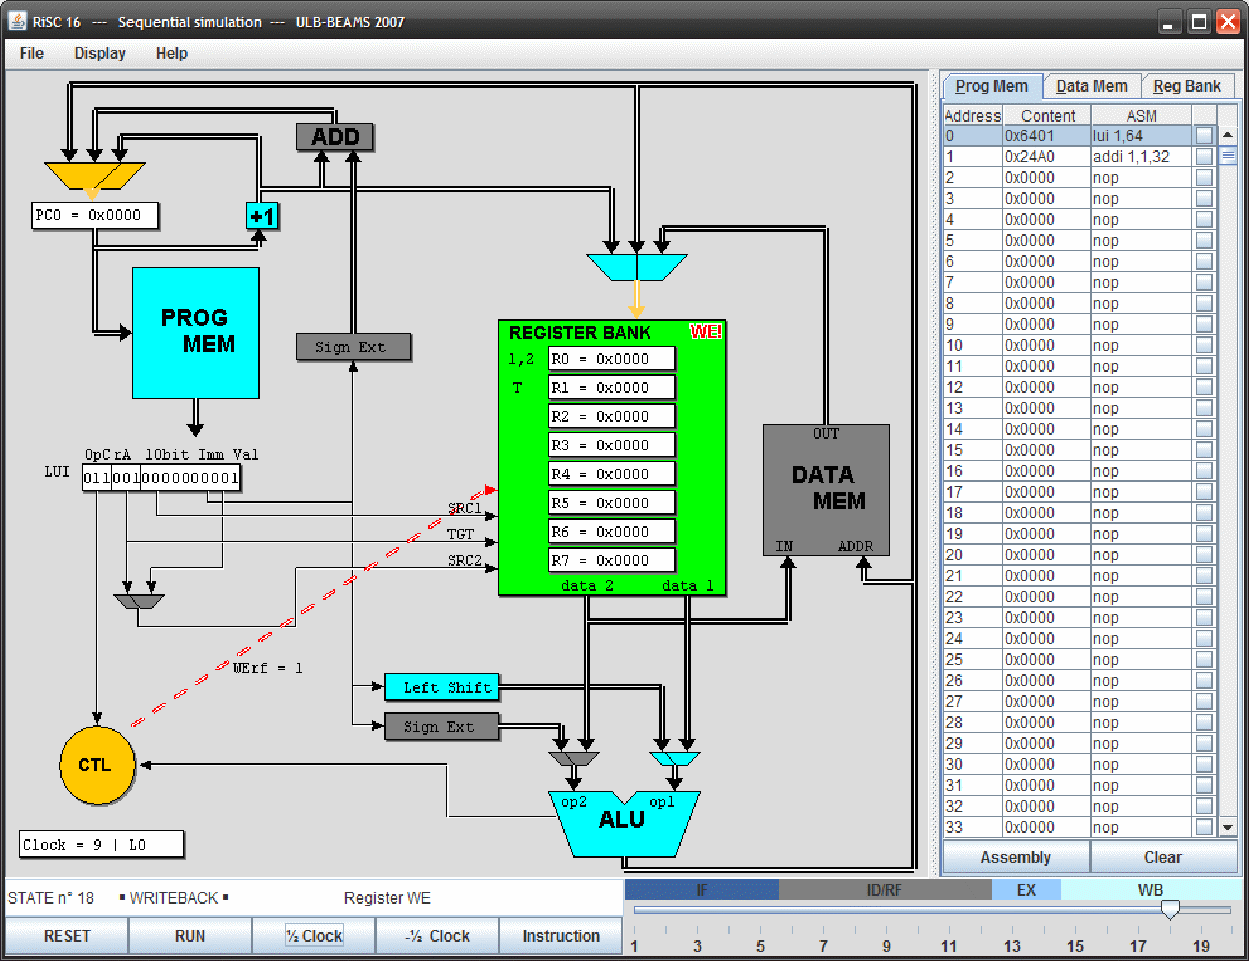
\includegraphics[width=16cm]{RiSC16_enonce_1_html_m16049efd.png}
	\end{center}
\caption{RiSC16 -- Simulation view}
\label{fig:RISC}
\end{figure}
\newpage
The user interface has 4 zones:
\begin{itemize}
\item the lower part groups the interaction possibilities: buttons provide \textit{reinitialisation} (reset), \textit{execution} (run), \textit{half-cycle execution}, \textit{instruction execution} and \textit{undo last instruction} capabilities.
\item The text zone above displays general informations about instruction execution. The cursor on the right can be used to follow each step of instruction execution and can be used to jump at any step of this instruction.
\item The zone on the right shows and allows editing program and data memory. A third tab shows register, they can also be modified.
\item The central zone shows the microprocessor representation

\end{itemize}

%Au niveau de l’interface du simulateur, on distingue 3 zones :
%la zone inférieure comprend les différents moyens d’interaction. Les boutons permettent de réinitialiser l’état du processeur (reset), d’exécuter un programme jusqu’au prochain breakpoint (run), d’exécuter le programme par demi-coups d’horloge ou par instruction, d’annuler le dernier demi-coup d’horloge. 

%La zone de texte située juste au-dessus des boutons affiche les grandes lignes de ce qu’il se passe durant l’exécution de l’instruction. Le curseur sur la droite permet de suivre l’exécution d’une instruction au cours du temps et de revenir à n'importe quel moment de cette exécution ;

%la zone sur la droite permet de voir et d’éditer le contenu de la mémoire programme et de la mémoire de donnée. Un troisième onglet permet de modifier le contenu des registres ;

%la zone centrale comprend la représentation du microprocesseur.

%

\section{Processor description}

Several blocks are used in this microprocessor:
\begin{itemize}
\item Program memory (\verb!PROG MEM!) and Data memory (\verb!DATA MEM!) -- Harvard architecture
\item Internal register bank (\verb!Register Bank!) to store operands and computation results. Register 0 (\reg{0}) has a special meaning: it is a read only register containing the \verb!0! value. A write in \reg{0} has no effect.
\item The Arithmetic and Logic Unit (ALU) is used to execute the operations needed to execute instructions. Complement to 2 arithmetic is used. 4 operations are possible:
	\begin{enumerate}
	\item add two operands, used during \verb!ADD, ADDI, LW, SW!
	\item bitwise NAND of two operands, used obviously during \verb!NAND!
	\item no modification, result is \verb!OP1!, used during \verb!LUI, JALR!
	\item operand comparison, used during \verb!BEQ!
	\end{enumerate}
\item The Control Unit (\verb!CTL!) decodes the opcode and configure other blocks accordingly. It's synchronised on the clock and can be used for rising edge or falling edge operation.
\item The program counter \verb!PC0!
\item The instruction register
\item The incrementer \verb!+1!
\item The adder (\verb!ADD!) to compute the address for jumps (Branch with \verb!BEQ!)
\item The immediate value converter (left shift and sign extension)
\end{itemize}

Blocks are linked together using buses with width of 1, 3, 6, 10 or 16 bits. Control signals are:
\begin{itemize}
\item \verb!WE_rf!: write in register bank
\item \verb!FUNC_alu!: operation to use
\item \verb!Mux_rf!, \verb!Mux_alu! (1, 2), \verb!Mux_tgt!, \verb!Mux_pc! : select multiplexer input
\item \verb!WE_dmem!: write in data memory
\item \verb!PSEN! : read from program memory.
\item \verb!WE_PCO! : write data into \verb!PC0!.
\end{itemize}


%Détaillons les différents blocs constituant ce microprocesseur :
%la mémoire programme (PROG MEM) et la mémoire de données (DATA MEM) séparées, puisque c'est une architecture de Harvard ;
%le banc de registres internes (Register Bank) pour stocker les opérandes et les résultats des opérations; une particularité de ce banc de registres est que le registre 0 contient toujours 0 (une écriture dans ce registre n'a aucun effet);
%l'unité arithmétique et logique (ALU) pour exécuter les différentes opérations nécessaires à l'exécution des instructions. Ces opérations sont au nombre de 4 : addition des deux opérandes (ADD, ADDI, LW et SW), NAND bit à bit des deux opérandes (NAND), passage sans modification de l'opérande op1 (LUI et JALR) et comparaison des deux opérandes (BEQ);
%l’unité de contrôle (CTL) qui s’occupe de décoder l’opcode et de commander les autres blocs en leur envoyant des signaux de contrôle. Elle est synchronisée sur l’horloge et peut activer un signal de contrôle sur un flanc montant comme sur un flanc descendant.
%le Program Counter (PC0);
%le registre d'instruction (en dessous de la mémoire programme);
%l'incrémenteur (+1), qui incrémente le Program Counter dans le cas du déroulement séquentiel du programme;
%l'additionneur (ADD), qui calcule l'adresse dans le cas d'un branchement (BEQ);
%les blocs de conversion de valeurs immédiates (left shift et sign ext).
%Les différents blocs sont reliés entre eux par des bus pouvant avoir des tailles de 1, 3, 6, 10 ou 16 bits. Les différents signaux de contrôle sont :
%WE_rf : ordre d'écriture dans le banc de registre
%FUNC_alu : pour indiquer à l'ALU quelle opération effectuer
%Mux_rf, Mux_alu (1,2), Mux_tgt, Mux_pc : sélection de l'entrée active de chaque multiplexeur 
%WE_dmem : ordre d'écriture dans la mémoire de données.
%PSEN : ordre de lecture en mémoire de programme.
%WE_PCO : ordre d'écriture dans PC0 de la donnée présente à son entrée.

The instruction set has 8 elementary instructions. None of them can be replaced by any combination of other instructions and complex problems can be solved using only these 8 instructions.
This architecture is RISC at its fate.

\subsection{Instructions detailed description}
Each instruction and how to code it is described below.
\subsubsection{$\on{ADD} : R\left[ \on{regA} \right] \longleftarrow R\left[ \on{regB} \right] + R\left[ \on{regC} \right] $}
\begin{center}
	\begin{tabular}{b{1.2cm}p{8cm}}
	bits & %first line
	 \begin{tabular}{C{1.5cm}C{1.5cm}C{1.5cm}C{2cm}C{1.5cm}}
		3 & 3 & 3 & 4 & 3 \\
	 \end{tabular} 	 \\ 
	 %second line:
	ADD & 
	 \begin{tabular}{|C{1.5cm}|C{1.5cm}|C{1.5cm}|C{2cm}|C{1.5cm}|}
	 	\hline  000 & regA & regB & 0000& regC \\  \hline 
	 \end{tabular} \\ 
	\end{tabular} 
\end{center}

Adds content from \reg{B} with content from \reg{C} and writes result in \reg{A}.


\subsubsection{$\on{ADDI} \on{(ADD\; immediate)} : R\left[ \on{regA} \right] \longleftarrow R\left[ \on{regB} \right] + \on{immed} $}
\begin{center}
	\begin{tabular}{m{1.2cm}m{8cm}}
	bits & %first line
	 \begin{tabular}{C{1.5cm}C{1.5cm}C{1.5cm}C{3.5cm}}
		3 & 3 & 3 & 7 \\
	 \end{tabular} 	 \\ 
	 %second line:
	ADDI & 
	 \begin{tabular}{|C{1.5cm}|C{1.5cm}|C{1.5cm}|C{3.5cm}|}
	 	\hline  001 & regA & regB & signed immediate \\  \hline 
	 \end{tabular} \\ 
	\end{tabular} 
\end{center}

Adds content from \reg{B} with an immediate 7-bit signed constant (-64 to 63) extended to 16-bits. Writes result in \reg{A}.

\subsubsection{$\on{NAND} : R\left[ \on{regA} \right] \longleftarrow \on{NOT}\left( R\left[ \on{regB} \right] \& R\left[ \on{regC} \right]\right) $}
\begin{center}
	\begin{tabular}{m{1.2cm}m{8cm}}
	bits & %first line
	 \begin{tabular}{C{1.5cm}C{1.5cm}C{1.5cm}C{2cm}C{1.5cm}}
		3 & 3 & 3 & 4 & 3 \\
	 \end{tabular} 	 \\ 
	 %second line:
	NAND & 
	 \begin{tabular}{|C{1.5cm}|C{1.5cm}|C{1.5cm}|C{2cm}|C{1.5cm}|}
	 	\hline  010 & regA & regB & 0000 & regC \\  \hline 
	 \end{tabular} \\ 
	\end{tabular} 
\end{center}

Bitwise NAND using content from \reg{B} and \reg{C}. Writes result in \reg{A}.

\subsubsection{$\on{LUI} \on{(Load Upper Immediate)} : R\left[ \on{regA} \right] \longleftarrow \on{immed<<6} \& \on{0xFFC0} $}
\begin{center}
	\begin{tabular}{m{1.2cm}m{8cm}}
	bits & %first line
	 \begin{tabular}{C{1.5cm}C{1.5cm}C{5cm}}
		3 & 3 & 10 \\
	 \end{tabular} 	 \\ 
	 %second line:
	LUI & 
	 \begin{tabular}{|C{1.5cm}|C{1.5cm}|C{5cm}|}
	 	\hline  011 & regA & immediate (0 to 0x3FF) \\  \hline 
	 \end{tabular} \\ 
	\end{tabular} 
\end{center}

Immediate 10-bit constant sign extended and written in \reg{A}.

\subsubsection{$\on{LW} \on{(Load~ Word)} : R\left[ \on{regA} \right] \longleftarrow \on{Mem}\left[ R\left[ \on{regB} \right] +\on{immed} \right] $}
\begin{center}
	\begin{tabular}{m{1.2cm}m{8cm}}
	bits & %first line
	 \begin{tabular}{C{1.5cm}C{1.5cm}C{1.5cm}C{5cm}}
		3 & 3 & 3 & 7 \\
	 \end{tabular} 	 \\ 
	 %second line:
	LW & 
	 \begin{tabular}{|C{1.5cm}|C{1.5cm}|C{1.5cm}|C{5cm}|}
	 	\hline  100 & regA & regB & signed immediate \\  \hline 
	 \end{tabular} \\ 
	\end{tabular} 
\end{center}

Reads a word in memory at address (\reg{B}+immediate). Immediate 7-bit constant is sign extended to 16-bit before the addition. This is an indirect addressing with offset.

\subsubsection{$\on{SW} \on{(Store~ Word)} : R\left[ \on{regA} \right] \longrightarrow \on{Mem}\left[ R\left[ \on{regB} \right] +\on{immed} \right] $}
\begin{center}
	\begin{tabular}{m{1.2cm}m{8cm}}
	bits & %first line
	 \begin{tabular}{C{1.5cm}C{1.5cm}C{1.5cm}C{5cm}}
		3 & 3 & 3 & 7 \\
	 \end{tabular} 	 \\ 
	 %second line:
	SW & 
	 \begin{tabular}{|C{1.5cm}|C{1.5cm}|C{1.5cm}|C{5cm}|}
	 	\hline  101 & regA & regB & signed immediate \\  \hline 
	 \end{tabular} \\ 
	\end{tabular} 
\end{center}

Writes the content of \reg{A} to memory at address (\reg{B}+immediate). Immediate 7bit constant is sign extended to 16bit before the addition. This is an indirect addressing with offset.


\subsubsection{$ \on{BEQ} \on{(Branch\;if\; EQual)}$ :\\ $\on{if} R\left[ \on{regA} \right]== R\left[ \on{regB} \right] \allowbreak \left\lbrace \on{PC}\longleftarrow \on{PC+1+immed} \right\rbrace\on{else} \left\lbrace\on{PC}\longleftarrow \on{PC+1} \right\rbrace $}
\begin{center}
	\begin{tabular}{m{1.2cm}m{8cm}}
	bits & %first line
	 \begin{tabular}{C{1.5cm}C{1.5cm}C{1.5cm}C{5cm}}
		3 & 3 & 3 & 7 \\
	 \end{tabular} 	 \\ 
	BEQ & 
	 %second line:
	 \begin{tabular}{|C{1.5cm}|C{1.5cm}|C{1.5cm}|C{5cm}|}
	 	\hline  110 & regA & regB & signed immediate \\  \hline 
	 \end{tabular} \\ 
	\end{tabular} 
\end{center}

Compares content of \reg{A} and \reg{B}. If equal, $\on{PC}$ is updated to $\on{PC}_{\on{BEQ}}+1+\on{immed(extended)}$ else \verb!PC! is just incremented by 1.


\subsubsection{$\on{JALR} \on{(Jump~ And ~Link ~using ~Register)} : \on{PC}\longleftarrow R\left[ \on{regB} \right], R\left[ \on{regA} \right]\longleftarrow \on{PC+1} $}
\begin{center}
	\begin{tabular}{m{1.2cm}m{8cm}}
	bits & %first line
	 \begin{tabular}{C{1.5cm}C{1.5cm}C{1.5cm}C{5cm}}
		3 & 3 & 3 & 7 \\
	 \end{tabular} 	 \\ 
	 %second line:
	JALR & 
	 \begin{tabular}{|C{1.5cm}|C{1.5cm}|C{1.5cm}|C{5cm}|}
	 	\hline  111 & regA & regB & 0 \\  \hline 
	 \end{tabular} \\ 
	\end{tabular} 
\end{center}

Jumps to address stored in \reg{B}. Writes \verb!PC+1! in \reg{A}. This is a call with saved return address.
%\begin{tabular}{c |cp{3cm}|cp{3cm}|cp{3cm}|cp{4cm}|cp{3cm}|}
% & 3 bits & 3 bits & 3 bits & 4 bits & 3 bits \\ 
%\cline{2-6}
%ADD & 000 & regA & regB & 0 & regC \\ 
%\cline{2-6}
%\end{tabular} %Le jeu d’instruction de ce processeur est constitué des 8 instructions présentées ci-dessous. Ce processeur illustre la philosophie RISC poussée à son maximum de simplicité. En effet, ces instructions sont élémentaires, mais elles sont suffisantes pour résoudre des problèmes complexes, et aucune instruction ne peut être remplacée par une combinaison des autres.
%1. ADD : R[regA] ← R[regB] + R[regC]
%
%Addition du contenu de regB et regC. Ecriture du résultat dans regA.

%2. ADDI (ADD Immediate) : R[regA] ← R[regB] + immed
%
%Addition du contenu de regB et d’une constante immédiate 7bits étendue à 16 bits. Ecriture du résultat dans regA.
%
%3. NAND : R[regA] ← NOT(R[regB] & R[regC])
%
%Opération NAND bit-à-bit entre les contenus de regB et regC. Ecriture du résultat dans regA.
%
%4. LUI (Load Upper Immediate) : R[regA] ← immed & 0xffc0
%
%Ecriture d’une constante immédiate 10 bits étendue sur 16 bits dans regA.
%
%5. LW (Load Word) : R[regA] ← Mem[R[regB] + immed]
%
%Ecriture dans regA de la valeur lue en mémoire de données à l’adresse formée par l’addition du contenu de regB et d’une constante immédiate 7 bits étendue à 16 bits (adressage indirect avec offset)
%
%6. SW (Store Word) : R[regA] → Mem[R[regB] + immed]
%
%Ecriture en mémoire de donnée du contenu de regA, à l’adresse donnée par l’addition du contenu de regB et d’une constante immédiate étendue sur 16 bits (adressage indirect avec offset)
%
%7. BEQ (Branch if EQual) : if (R[regA] == R[regB] ) {PC ← PC+1+immed} else  {PC ← PC+1}
%
%Comparaison du contenu de regA et de regB. En cas d’égalité, le PC vaut PCBEQ+1+imm(extend), sinon, il vaut PCBEQ+1
%
%8. JALR (Jump And Link using Register) : PC ← R[regB] , R[regA]←PC+1
%
%Saut à l’adresse contenue dans regB. Ecriture dans regA de PC+1. Correspond à un appel de fonction avec stockage de l'adresse de retour dans le Registre désigné

\subsection{Pseudo Instructions}

Other (pseudo-)instructions can be used:
\subsubsection{\texttt{NOP}}
\verb!NOP = ADD 0,0,0!

This instruction does nothing because writing to \reg{0} has no effect (\reg{0} is \textit{read only}).

\subsubsection{\texttt{RESET}}
\verb!RESET = JALR 0,0!

This pseudo instruction changes \verb!PC! to \verb!0! and thus resets the processor. Registers and data memory remain unchanged.

\subsubsection{\texttt{MOVI}}
\verb!MOVI rx,imm(16bits) = LUI rx, immH(10bits); ADDI rx,rx,immL(6bits)!

This pseudo instruction can be used to load a 16-bit immediate constant to \reg{(rx)}. Two instructions are used to perform this pseudo instruction. \verb!LUI! loads the upper 10 bits and \verb!ADDI! loads the 6 lower bits. To avoid any unexpected side effect during assembly, be sure to add a \verb!NOP! after this instruction. The \verb!NOP! will be replaced by the \verb!ADDI! instruction.

Depending on their size, immediate constants are extended to 16 bits:
\begin{itemize}
\item Immediate 7bit signed constants (from -64 to 63) are sign-extended to 16 bits before they are used.
\begin{center}
\begin{tabular}{c *{16}{C{0.5cm}}}
%\hline 
bit & 15 & 14 & 13 & 12 & 11 & 10 & 9 & 8 & 7 & 6 & 5 & 4 & 3 & 2 & 1 & 0 \\ 
\cline{2-17}
ADDI & \multicolumn{3}{|c}{001} & \multicolumn{3}{|c}{regA}& \multicolumn{3}{|c}{regB}& \multicolumn{7}{|c|}{immed-7} \\ 
\cline{2-17}
% &\tabnode{} &  \tabnode{} &  \tabnode{ 13 } &  \tabnode{ 12 } &  \tabnode{ 11 } &  \tabnode{ 10 } &  \tabnode{ 9 } &  \tabnode{ 8 } &  \tabnode{ 7 } &  \tabnode{ 6 } &  \tabnode{ 5 } &  \tabnode{ 4 } &  \tabnode{ 3 } &  \tabnode{ 2 } &  \tabnode{ 1 } &  \tabnode{ 0 } 
%\\
& & & & & & & & & &\tabnode{}&\tabnode{}&\tabnode{}&\tabnode{}&\tabnode{}&\tabnode{}&\tabnode{}
\\
\\
&\tabnode{}&\tabnode{}&\tabnode{}&\tabnode{}&\tabnode{}&\tabnode{}&\tabnode{}&\tabnode{}&\tabnode{}&\tabnode{}&\tabnode{}&\tabnode{}&\tabnode{}&\tabnode{}&\tabnode{}&\tabnode{}\\
\cline{2-17}
operand & \multicolumn{16}{|c|}{} \\
\cline{2-17}
%
\begin{tikzpicture}[overlay,>=stealth]
% Define the circle paths
\draw   [->]  (1.north)+(0,0.3) |- ++(0,-0.5) -| (8.south);%+(-0.7,1.3);%+(-0.7,1.3)
\draw  [->](1.north)+(0,0.3) |- ++(0,-0.5) -|  (9.south) ;
\draw  [->](1.north)+(0,0.3) |- ++(0,-0.5) -|  (10.south) ;
\draw  [->](1.north)+(0,0.3) |- ++(0,-0.5) -|  (11.south) ;
\draw  [->](1.north)+(0,0.3) |- ++(0,-0.5) -|  (12.south) ;
\draw  [->](1.north)+(0,0.3) |- ++(0,-0.5) -|  (13.south) ;
\draw  [->](1.north)+(0,0.3) |- ++(0,-0.5) -|  (14.south) ;
\draw  [->](1.north)+(0,0.3) |- ++(0,-0.5) -|  (15.south) ;
\draw  [->](1.north)+(0,0.3) |- ++(0,-0.5) -|  (16.south) ;
\draw  [->](1.north)+(0,0.3) |- ++(0,-0.5) -|  (17.south) ;
%
%
\draw  [->](2.north)+(0,0.3) |- ++(0,-0.5) -|  (18.south) ;
\draw  [->](3.north)+(0,0.3) |- ++(0,-0.5) -|  (19.south) ;
\draw  [->](4.north)+(0,0.3) |- ++(0,-0.5) -|  (20.south) ;
\draw  [->](5.north)+(0,0.3) |- ++(0,-0.5) -|  (21.south) ;
\draw  [->](6.north)+(0,0.3) |- ++(0,-0.5) -|  (22.south) ;
\draw  [->](7.north)+(0,0.3) |- ++(0,-0.5) -|  (23.south) ;
\end{tikzpicture}
\end{tabular}
\end{center}
%
\item Immediate 10bit constants are unsigned numbers from 0 to 1023.
%
\setcounter{nodecount}{0}
\begin{center}
\begin{tabular}{c *{16}{C{0.5cm}}}
%\hline 
bit & 15 & 14 & 13 & 12 & 11 & 10 & 9 & 8 & 7 & 6 & 5 & 4 & 3 & 2 & 1 & 0 \\ 
\cline{2-17}
LUI & \multicolumn{3}{|c}{011} & \multicolumn{3}{|c}{regA}& \multicolumn{10}{|c|}{immed-10} \\ 
\cline{2-17}
% &\tabnode{} &  \tabnode{} &  \tabnode{ 13 } &  \tabnode{ 12 } &  \tabnode{ 11 } &  \tabnode{ 10 } &  \tabnode{ 9 } &  \tabnode{ 8 } &  \tabnode{ 7 } &  \tabnode{ 6 } &  \tabnode{ 5 } &  \tabnode{ 4 } &  \tabnode{ 3 } &  \tabnode{ 2 } &  \tabnode{ 1 } &  \tabnode{ 0 } 
%\\
& & & & & & &\tabnode{} &\tabnode{} &\tabnode{} &\tabnode{}&\tabnode{}&\tabnode{}&\tabnode{}&\tabnode{}&\tabnode{}&\tabnode{}\\
\\
\\
\cline{12-17}
\multicolumn{11}{c}{} &\multicolumn{1}{|c}{\tabnode{0}} &\tabnode{0} &\tabnode{0} &\tabnode{0} &\tabnode{0} &\multicolumn{1}{c|}{\tabnode{0}} \\
\cline{12-17}
&\tabnode{}&\tabnode{}&\tabnode{}&\tabnode{}&\tabnode{}&\tabnode{}&\tabnode{}&\tabnode{}&\tabnode{}&\tabnode{}&\tabnode{}&\tabnode{}&\tabnode{}&\tabnode{}&\tabnode{}&\tabnode{}\\
\cline{2-17}
operand & \multicolumn{16}{|c|}{} \\
\cline{2-17}
%
\begin{tikzpicture}[overlay,>=stealth]
% Define the circle paths
\draw   [->]  (1.north)+(0,0.2) -| ++(0,-0.1) -|  (17.south);%+(-0.7,1.3);%+(-0.7,1.3)
\draw  [->](2.north)+(0,0.2)  -| ++(0,-0.2) -|  (18.south) ;
\draw  [->](3.north)+(0,0.2)  -| ++(0,-0.3) -|   (19.south) ;
\draw  [->](4.north)+(0,0.2)  -| ++(0,-0.4) -|  (20.south) ;
\draw  [->](5.north)+(0,0.2)  -| ++(0,-0.5) -|  (21.south) ;
\draw  [->](6.north)+(0,0.2)  -| ++(0,-0.6) -|  (22.south) ;
\draw  [->](7.north)+(0,0.2)  -| ++(0,-0.7) -|  (23.south) ;
\draw  [->](8.north)+(0,0.2)  -| ++(0,-0.8) -|  (24.south) ;
\draw  [->](9.north)+(0,0.2)  -| ++(0,-0.9) -|  (25.south) ;
\draw  [->](10.north)+(0,0.2)  -| ++(0,-1) -|  (26.south) ;
%
%
\draw  [->](11.south)+(0,-0.1) --  (27.south) ;
\draw  [->](12.south)+(0,-0.1) --  (28.south) ;
\draw  [->](13.south)+(0,-0.1) --  (29.south) ;
\draw  [->](14.south)+(0,-0.1) --  (30.south) ;
\draw  [->](15.south)+(0,-0.1) --  (31.south) ;
\draw  [->](16.south)+(0,-0.1) --  (32.south) ;
\end{tikzpicture}
\end{tabular}
\end{center}
%
\end{itemize}

\subsubsection{\texttt{HALT}}
This pseudo instruction stops the simulator.
\subsection{Instruction execution}
All instructions are executed in 4 stages:
\begin{enumerate}
\item \verb!IF! \textit{Instruction Fetch}: instruction is copied from the program memory to the instruction register
\item \verb!ID/RF! \textit{Instruction Decode/Register Fetch}: instruction decoding and operand extraction
\item \verb!EX!	\textit{Execute}: instruction execution in the ALU
\item \verb!WR! \textit{Write Back}: result saving or data memory access
\end{enumerate}

As the RiSC-16 is a RISC architecture\footnote{Incredible, isn't it?}, all instructions have the same execution time, which is 20 half clock-cycles. Control signals are activated considering the slowest instruction, which is \verb!BEQ!. The details of a machine cycle (execution of one instruction) are detailed in Table \vref{tab:stages}.

\setlength{\tabcolsep}{3pt} %no extra space in cells to keep constant tabular width
\begin{landscape}
\begin{table}[]
	\begin{center}
		\begin{small}
			%\begin{turn}{90}
			\hspace*{-1.5cm}
				\begin{tabular}{ll|cc|llll|c|lllll}
					\toprule
					\multicolumn{2}{c|}{Stage:} & \multicolumn{2}{c|}{IF} & \multicolumn{4}{c|}{ID/RF} & EX & \multicolumn{5}{c}{WB} \\ 
					\multicolumn{2}{c|}{Half-cycle:} & 
					 1--2--3  & 4--5  & 6--7  & 8 & 9 & 10--11--12  & 13--14 & 15--16  & 17 & 18 & 19 & 20 \\ 
					\midrule
					%\hline 
					%0 &0 & 1& 2& 3& 4& 5& 6& 7& 8& 9& 10& 11& 12 \\
					ADD & 000 & ROM & IR & CTL+RF(src1) & CTL+Mux\_RF+RF(src1) & Mux\_RF & RF(src2) & ALU &  & Mux\_PC & RF+Mux\_PC & RF+PC & RF+PC \\ 
					ADDI & 001 & ROM & IR & CTL+RF(src1)+Sign\_ext & CTL+RF(src1) &  &  & ALU &  & Mux\_PC & RF+Mux\_PC & RF+PC & RF+PC \\ 
					NAND & 010 & ROM & IR & CTL+RF(src1) & CTL+Mux\_RF+RF(src1) & Mux\_RF & RF(src2) & ALU &  & Mux\_PC & RF+Mux\_PC & RF+PC & RF+PC \\ 
					LUI & 011 & ROM & IR & CTL+Left\_Shift & CTL &  &  & ALU &  & Mux\_PC & RF+Mux\_PC & RF+PC & RF+PC \\ 					
					LW & 100 & ROM & IR & CTL+RF(src1)+Sign\_ext & CTL+RF(src1) & & & ALU & datam & datam+Mux\_PC & RF+Mux\_PC & RF+PC & RF+PC \\
					SW & 101 & ROM & IR & CTL+RF(src1)+Sign\_ext & CTL+Mux\_RF+RF(src1) & Mux\_RF & RF(src2) & ALU & datam & datam+Mux\_PC & Mux\_PC & PC & PC \\ 
					BEQ & 110 & ROM & IR & CTL+RF(src1)+Sign\_ext & CTL+Mux\_RF+RF(src1)+ADD & Mux\_RF+ADD & RF(src2) & ALU & CTL& CTL+Mux\_PC & Mux\_PC & PC & PC \\ 
					%NAND & 010 & ROM & IR & CTL+RF(src1) & CTL+Mux\_RF+RF(src1) & Mux\_RF & RF(src2) & ALU &  & Mux\_PC & RF+Mux\_PC & RF+PC & RF+PC \\
					JALR & 111 & ROM & IR & CTL+RF(src1) & CTL+RF(src1) & & & ALU &  & Mux\_PC & RF+Mux\_PC & RF+PC & RF+PC \\ 
					\bottomrule
				\end{tabular} 
			%\end{turn}
		\end{small}
	\end{center}
\caption{Detailed instruction processing}
\label{tab:stages}
\end{table}
\end{landscape}
%D’autres instructions appelées pseudo-instructions peuvent être utilisées :
%NOP = ADD 0,0,0 : cette pseudo instruction ne fait rien puisqu’elle place le résultat dans le registre 0 qui n’est pas accessible en écriture.
%RESET = JALR 0,0 : cette pseudo instruction remet le PC à une valeur nulle.
%MOVI rx,imm(16bits) = LUI rx,immH(10bits) suivi de ADDI rx,rx,immL(6bits) Cette pseudo instruction permet de charger une constante immédiate de 16 bits. Elle est une succession d’une instruction LUI qui charge les bits de poids forts et de l’instruction ADDI qui charge les bits de poids faibles sous forme des 6 bits significatifs d'une constante 7 bits positive.

%Selon leur nombre de bit, les constantes immédiates sont étendues à 16 bits de différentes manières :
%Les constantes immédiates de 7 bits sont des nombres signés compris entre -64 et 63. On remarque l'extension du bit de signe pour faire une constante 16 bits signée.

%Les constantes immédiates de 10 bits sont des nombres non-signés de 0 à 1023.





%Une instruction s’exécute en 4 étapes :
%IF (Instruction Fetch) : extraction de l’instruction depuis la mémoire programme vers le registre d'instruction,
%ID/RF (Instruction Decode/ Register Fetch) : décodage de l'instruction et extraction des opérandes,
%EX (Execute) : exécution de la fonction au niveau de l’ALU,
%WB (WriteBack) : sauvegarde du résultat ou l'accès en mémoire de données.

%Comme l’architectur% du RiSC-16 est de type RISC, toutes les instructions prennent le même temps d’exécution, qui est de 20 demi-coups d’horloge. Les instants où les signaux de contrôle seront activés, sont donc calibrés sur l’instruction prenant le temps d’exécution le plus long, c’est-à-dire, l’instruction BEQ. La décomposition d’un cycle machine (temps d’exécution d’une instruction) est donnée à la figure suivante. La ligne du bas donne le numéro du ½ coup d'horloge.

\section{Simulation dynamics}
Most elements are asynchronous, which means that no register buffers data between blocks but the control unit:
\begin{itemize}
\item is synchronous to the clock
\item provides control signal \verb!WE! just after clock rising edges for write operations to the \verb!PC!, to the register bank and to the data memory.
\item provides a read in ROM signal \verb!PSEN! just after a clock rising edge, which provides a synchronisation on instruction reading. An instruction is extracted each 20 \textonehalf cycles precisely.
\end{itemize}
%Dynamique de la simulation
%La majorité des éléments travaillent de manière asynchrone, ce qui veut dire qu’entre deux éléments, il n’y a pas de registre (latch) intermédiaire contrôlé par l’horloge ou un signal de contrôle. Par contre, l’unité de contrôle
%est synchronisée sur l’horloge
%fournit des signaux de contrôle WE juste après les flancs d'horloge pour les opérations d'écriture dans le PC, le banc de registre, ainsi que la mémoire de données
%fournit un signal de lecture en ROM (PSEN) juste après un flanc d'horloge ce qui, globalement introduit une synchronisation au niveau de l’instruction (il y a une extraction d'instruction tous les 20 ½ cycles précisément)

The simulator aims at exposing in detail the internal processor behaviour during execution. To highlight and ease understanding, three colors %\footnote{I tried to use color which can be distinguished in BW}
 are used for different states:
\begin{itemize}
\item {\color{green}{Green}}: used to show that the block is busy: input data is stable and the block is processing them. This transient state ends after the propagating time in the block. This state is irrelevant for busses.
\item {\color{orange}{Orange}}: this states follows the previous one. The block has processed data and the result is available. Output signals also take that stable state.
\item Default color: this color is used for ``has been used'' and for default state. Default state means that the block has not yet received data for the current instruction. State ``has been used'' means that the block has provided its result to the other blocks and will not do anything until the next instruction.
\end{itemize}

Figure \vref{fig:chg} shows the different states and the associated colors. Lines represent output buses for a specific block.
\begin{figure}[h!]
	\begin{center}
		\tikzstyle{every path}+=[thick, sharp corners]
		%\tikzset{timing/d/background/.style={font=\ttfamily,fill=green}}
		%\tikzset{timing/u/background/.style={font=\ttfamily,fill=orange}}
		\begin{tikztimingtable}
%						& 	transitional	stable	has been used
			element n   &	[green]2D{}; 2D[orange]4D;[black] 4D{}\\
			element n+1	&	4D;[green] 2D{} 2D; [orange]4D{} \\
%WR			&	7.2L2H6L2H2L\\
\extracode
\tablerules
\vertlines[help lines]{0,4,8,12}
\end{tikztimingtable}
	\end{center}
\caption{Transitional, stable and ``Has been used'' states.}
\label{fig:chg}
\end{figure}

After opcode decoding, unused blocks in the instruction will be greyed. See \verb!ADD! and DATA MEM on Figure \vref{fig:RISC}. It's not a specific state but it is used to de-emphasize unused blocks to ease user thoughts by highlighting only relevant blocks.

Any greyed block will provide a signal computed from its input but the actual value is useless, and so is not displayed. 
%Le but du simulateur est de montrer en détail ce qui se passe à l'intérieur du processeur lors de l'exécution de ses instructions. Pour cela, un code de couleurs est utilisé pour mettre en évidence les éléments qui fournissent aux éléments suivants des données utiles à l’instruction en cours. Trois couleurs représentent les différents états :
%Vert signifie que le bloc est occupé : des données sont stables aux entrées et le bloc est en train de les traiter. Dès lors, cet état est transitoire, il se termine après le temps de propagation du bloc. Un tel état n’existe pas pour les bus.
%Orange : cet état suit toujours le précédent. Le bloc a fini de traiter les données et elles sont disponibles à la sortie. Les signaux de sortie deviennent également oranges. Cet état peut être décrit comme stable.
%Couleur par défaut : cette couleur est utilisée pour deux états: l’état par défaut et l’état « a été utilisé ». L’état par défaut signifie que l’élément n’a pas encore reçu de données utiles pour l’instruction en cours. L’état « a été utilisé » veut dire que l’élément a fourni des données utiles aux blocs suivants et qu’il ne jouera plus aucun rôle pour l’instruction en court.
%La figure suivante illustre les différents états et les couleurs correspondantes d’un élément. Les lignes continues représentent le bus de sortie de l’élément considéré.

%Après le décodage de l’opcode, les blocs qui ne vont pas servir lors de la suite de l’exécution de l’instruction sont grisés. C’est le cas des blocs ADD, DATAMEM… de la capture d’écran. Il ne s’agit pas d’un état précis dans lequel se trouve l’élément, mais cela permet à l’utilisateur de différencier les éléments utiles à l’instruction de ceux qui ne le sont pas. Notons qu’un bloc grisé émet un signal, mais qui ne contient aucune information utile. Pour plus de clarté, ce signal n’est donc pas affiché.

%\textbf{Beware, Ogres!}

The simulation might show a synchronous behaviour because of instantaneous color change and aligned on clock edges to ease the simulator design and thus does not represent the behaviour of an actual implementation of the RiSC16. Most blocks have a propagating time lower than a half-period, as shown on Figure \vref{fig:chg}.

\section{The Simulator}

The assembly program can be loaded into the simulator from two sources:
\begin{itemize}
\item Writing instruction directly in the ASM column in ``Program memory'' window. To update the program memory with the modified instructions, use the ``assembly'' button. The pseudo instruction \verb!MOVI! will be replaced by two instructions so an empty line must follow this instruction.
\item Importing an external file using the ``File import ROM'' menu.
\end{itemize}

Several features are available when editing your program in an external file:
\begin{itemize}
\item Comments: anything after ``//'' on a single line
\item Any hexadecimal constant must begin with the ``\verb!0x!'' notation.
\item Place instruction at specific address: ``@'' followed by constant value must be added before the instructions
\item Labels: labels are defined using a name+``:'' at the beginning of a line
\end{itemize}

\newpage
Syntax for instructions is defined as:
\begin{center}
\texttt{{\color{blue}{label:}}<space>{\color{red}{opcode}}<space>{\color{green}{\textbf{field1}, field2, filed3}}<space>{\color{blue}{// comments}}}
\end{center}
Where:
%\parbox[b]{\linewidth}
%setitemize[0]{leftmargin=*}
\begin{itemize}
	\item  {\color{blue}{label:}} optional label
	\item  {\color{blue}{// comments}}: optional comment
	%\item [<space>]	
	\item {\color{red}{opcode}}:  opcode of the instruction (mandatory)
	\item {\color{green}{\textbf{field1}, 2, 3}}:	fields that can be register numbers, constants (instruction dependant)
\end{itemize}
%}

The program is assembled when the file is imported (menu ``File-Import ROM''). A program modified inside the program memory can also be saved to a file. Several files can be imported. Overlapping memory segments have the value of the last imported file. Importing and exporting RAM is also possible.
%Attention, la simulation pourrait vous faire penser que tous les éléments sont synchrones, à cause du fait que les changements de couleurs sont brutaux et alignés sur les flancs d'horloge, pour faciliter la représentation, mais il n’en est rien. La plupart des éléments sont asynchrones, avec un temps de propagation nécessairement inférieur à la demi-période d'horloge, comme le montre la figure ci-dessus
%Le simulateur
%Le programme en assembleur peut être introduit dans le simulateur deux manières :
%Ecriture des instructions dans colonne ASM de la fenêtre "Program Memory". Il faut dans ce cas cliquer sur le bouton assemblage pour traduire la colonne assembleur en binaire et mettre à jour le contenu de la mémoire. Attention, la pseudo instruction MOVI sera traduite en deux instructions, il faut donc laisser la ligne suivante vide dans le tableau.
%Edition d'un fichier texte et chargement via le menu File-Import ROM
 
%Certaines fonctionnalités sont disponibles lors d’une écriture d’un programme dans un fichier texte :
%Ajout de commentaires : ceux-ci doivent être précédés de " // ".
%Placement d’instruction à une adresse précisée : l’adresse doit être précédée de « @ » et placée au dessus des instructions.
%Valeurs écrites en hexadécimal : elles doivent être précédées de " 0x ". Cette notation peut également être utilisée dans la fenêtre "Program Memory".
%Utilisation des labels qui sont d’une grande utilité, en particulier pour les instructions de branchement. Le label doit être placé en début de ligne et suivi de ": "
%
%La syntaxe d’une instruction est donc la suivante :
%
%label:<espace>opcode<espace>champ1, champ2, champ3<espace>// commentaires
%
%Le nombre de champs dépend de l’instruction. Pour les instructions de branchement, le champ3 peut être le nom d'un label au lieu d’une valeur immédiate.

%L’assemblage du programme contenu dans le fichier texte a lieu lors de l’importation de ce dernier (menu File-Import ROM). Un programme écrit dans la fenêtre "Program Memory" peut également être sauvé dans un fichier texte. Plusieurs fichiers peuvent être importés. Lorsque des instructions sont situées à la même adresse, l’instruction du dernier fichier importé sera placée à cette adresse. L’importation et la sauvegarde est aussi disponible pour le contenu de la RAM. 
%Un exemple de fichier texte est donné à la figure suivante.
An example is given in Listing \vref{code:asm}.

\lstset{numbers=left, numberstyle=\tiny, stepnumber=5, numbersep=5pt, captionpos=b,style=customasm}
\begin{lstlisting}[float=h!,caption=Example code,label=code:asm,style=customasm]
		addi 	2,0,1	
		sw   	2,1,0
		addi 	1,1,1
		sw   	2,1,0			
		addi 	1,1,1
		add  	3,2,2
		sw   	3,1,0
		addi 	1,1,1
		addi 	7,0,7	
loop: 		beq  	7,0,end
		lw	2,1,-2
		add 	3,3,2	
		sw   	3,1,0
		addi 	1,1,1
		addi 	7,7,-1
		beq  	0,0,loop
end: 		halt
\end{lstlisting}
%\label{code:asm}

\newpage

\section{Manipulation}




\begin{Q}
Explain what is the example on listing \vref{code:asm} doing? Detail the state of registers and the state of the \verb!PC! after each instruction.
%\vspace{5cm}
\end{Q}

\begin{Q}
Load \verb!exemple1.txt! and run the simulation. Explain the internal behaviour for each instruction.
%\vspace{5cm}
\end{Q}

\begin{Q}
Using the graph in annexe \vref{an:graph}, draw the chronogram for the \verb!BEQ! instruction. Signals on the graph are output of blocks of the processor.
%\vspace{5cm}
\end{Q}


%For the following exercises, an online verification tool is available to run automated tests on your code. 
For each of the exercises \ref{Q:4}--\ref{Q:9}, you can automagically test your code against a set of \textit{test vectors} (listed in section \ref{sec:vectors}) using the ``\textbf{\ovt}'' at address: 
\begin{center}
	\href{http://164.15.75.7:80}{http://164.15.75.7:80}
\end{center}
Read this handout to the end to get a glimpse on its capabilities and to understand how to use it.
\begin{Q}
	%Q
	\label{Q:4}
	Write\footnote{\label{assign}And test it using the ``\ovt{}'', some results will be included in the quotation of these labs, read further for more details.} a program which shifts to the left the content of \reg{5}.
	%\label{Q:1}
	\reponse{}%R
\end{Q}

\begin{Q}
	%Q
	Write\footref{assign} a program which extracts the most significant bit from \reg{1} and stores the value (0/1) in \reg{7}. %The bit to extract is stored in \reg{7}.
	%\label{Q:1}
	\reponse{}%R
\end{Q}

\begin{Q}
	%Q
	Write\footref{assign} a program which shifts to the left a 32-bit value stored in \reg{6}(MSB), \reg{5}. %\reg{5} must be initialised from \reg{1}.
	%\label{Q:1}
	\reponse{}%R
\end{Q}



\begin{Q}
Write\footref{assign} a program which adds the unsigned content of \reg{1} and \reg{2} and writes the result in \reg{3} and the carry bit in \reg{4}.
%\vspace{5cm}
\end{Q}

%\begin{Q}
%	%Q
%	Write a program which adds the unsigned content 
%	\label{Q:1}
%	\reponse{}%R
%\end{Q}

%\begin{Q}
%Transform the program into a function. We suppose that the call will be done using the \verb!JALR! instruction which stores the return address into \reg{7}.
%%\vspace{5cm}
%\end{Q}

%bit extraction
%shift 
%add

%\begin{Q}
%	%Q
%	Left shift on 64 bits
%	\label{Q:1}
%	\reponse{}%R
%\end{Q}

\begin{Q}
	%Q
	%32b add
	Write\footref{assign} a program which adds the unsigned content of 32-bit numbers stored in \reg{4}(MSB), \reg{3} and \reg{6}(MSB), \reg{5} and writes the result in \reg{4}(MSB), \reg{3}.

	\label{Q:32b}
	\reponse{}%R
\end{Q}

\begin{Q}
\label{Q:9}
Write\footref{assign} a program which multiplies  the (unsigned) content of \reg{1} and \reg{2} and writes the result into \reg{4}(MSB), \reg{3}.
%\vspace{5cm}
\end{Q}

%\begin{Q}
%How would you modify this processor to make it synchronous ? What does this imply on the hardware and on the design ?
%%\vspace{5cm}
%\end{Q}

%\begin{Q}
%What are the ``must have" features missing in this processor, on the software and on the hardware side ? Express yourself and be creative.
%%\vspace{5cm}
%\end{Q}

\section{Code requirements/recommendations}
This section is for the multiplication but you can generalise to the other exercises according to the question formulation.
\label{ref:guidelines}
Be sure your code:
\begin{enumerate}
\item uses \reg{1} and \reg{2} for operands. Anything else will cause the tests to fail (because the verification program assumes operands are in \reg{1} and \reg{2} and nowhere else). \\ \textbf{Operands in correct registers}
\item uses \reg{4} and \reg{3} to store the result at the end of the execution. \reg{3} is the Least Significant Word. Same note as previous point, result \textbf{must} be in \reg{4}-\reg{3}. \\ \textbf{Result in correct registers}
\item initialises \reg{1} and \reg{2} using 2 \verb!movi! instructions at the beginning (any other initialisation method will cause the automatic tests to fail). This is necessary to ensure that your code will work with the verification tool if you use \verb!jalr! instructions for absolute jumps. These instructions will be replaced by \verb!nop! instructions during automatic testing. \\ \textbf{Use first instructions (2/4/8) to initialise your operands}
\item is writen knowing that the RAM is unaffected by any reset (you might get some bonus points by using this {feature} and creativity).
\item stops the simulator when the result is stored in \reg{4}-\reg{3} using a \verb!halt! instruction. \\\textbf{End your code}
\item works with the test vectors. If the test report marks some tests as failed but your simulator works, check the code at the beginning of the report against your code and \textbf{then} ask the assistant. Don't ask the assistant before checking (friendly warning).
\item has some comments.
\item does not use any illegal instruction and/or instruction with too big immediate values.
\item is not too greedy! (the verification tool stops any test after $10^7$ instructions)
\end{enumerate}

\newpage

\section{Test vectors}
\label{sec:vectors}
%Points awarded/signification:
This sections lists some usual test vectors to test the code you are writing for the different exercises. They are all integrated in the ``\ovt''.
\subsection{16b SLL}
%{\color{red} This exercise is removed from the quotation $\Longrightarrow$ 0 pt}
%\begin{itemize}
%\item 
%\item [1:] coding style (comments, readability)
%\item [-1:] error in code, by type of error
%\item [4×\%] of passed tests (see test vectors below)
%\end{itemize}
%\section{Test vectors}
%\label{sec:vect}
%All codes are automatically tested against:
input: \verb!reg5!, output: \verb!reg5!
{\ttfamily
\begin{itemize}
\item 0x0000 $\longrightarrow$ 0x0000
\item 0x0001 $\longrightarrow$ 0x0002
\item 0x8FFF $\longrightarrow$ 0x1FFE
\item 0x8000 $\longrightarrow$ 0x0000
\end{itemize}}
\subsection{Most Significant Bit extraction}
%\begin{itemize}
%\item 
%\item [1:] coding style (comments, readability)
%\item [-1:] error in code, by type of error
%\item [4×\%] of passed tests (see test vectors below)
%\end{itemize}
input: \verb!reg1!, output \verb!reg7!
{\ttfamily
\begin{itemize}
\item 0x0000  $\longrightarrow$ 0
\item 0x0001  $\longrightarrow$ 0
%\item 0x0100, 7  $\longrightarrow$ 0
%\item 0x0100, 8  $\longrightarrow$ 1
%\item 0x0100, 9  $\longrightarrow$ 0
\item 0x8000 $\longrightarrow$ 1
\item 0xFFFF $\longrightarrow$ 1
\end{itemize}}
\subsection{32b SLL}
%\begin{itemize}
%\item 
%\item [1:] coding style (comments, readability)
%\item [-1:] error in code, by type of error
%\item [4×\%] of passed tests (see test vectors below)
%\end{itemize}
input: \verb!reg6!(MSB), \verb!reg5!, output: \verb!reg6!(MSB), \verb!reg5!
{\ttfamily
\begin{itemize}
\item 0x00000000 $\longrightarrow$ 0x00000000
\item 0x00000001 $\longrightarrow$ 0x00000002
\item 0x00007FFF $\longrightarrow$ 0x0000FFFE
\item 0x00008000 $\longrightarrow$ 0x00010000
\item 0x80000000 $\longrightarrow$ 0x00000000
\item 0x80000001 $\longrightarrow$ 0x00000002
\item 0x0001FFFF $\longrightarrow$ 0x0003FFFE
\item 0x00042000 $\longrightarrow$ 0x00084000
\end{itemize}}

\subsection{16b+16b}
%\begin{itemize}
%\item 
%\item [1:] coding style (comments, readability)
%\item [-1:] error in code, by type of error
%\item [4×\%] of passed tests (see test vectors below)
%\end{itemize}
input: \verb!reg1!, \verb!reg2!; output: \verb!reg3!, carry: \verb!reg4!
{\ttfamily
\begin{itemize}
\item 0x0000 + 0x0000 = 0, 0x0000
\item 0x0001 + 0x0000 = 0, 0x0001
\item 0x0001 + 0x0001 = 0, 0x0002
\item 0x8000 + 0x4000 = 0, 0xC000
\item 0x7FFF + 0x7FFF = 0, 0xFFFE
\item 0xFFFF + 0xFFFF = 1, 0xFFFE
\item 0xFFFF + 0x0001 = 1, 0x0000
\item 0xFFFF + 0x0002 = 1, 0x0001
\end{itemize}}


\subsection{32b+32b}
This code will be evaluated using these elements:
\begin{itemize}
\item input: \verb!reg4!(MSB), \verb!reg3! and \verb!reg6!(MSB), \verb!reg5!; output: \verb!reg4!(MSB), \verb!reg3!
\item coding style (comments, readability)
\item errors in code
\item \% of passed tests (see test vectors below)
\end{itemize}
The mark will be expressed related to 2 (result is integer only, rounded down).
\newpage
\subsubsection{Test vectors for addition}
{\ttfamily
\begin{itemize}
\item 0x00000000 + 0x00000000 =  0x00000000
\item 0x00000001 + 0x00000000 =  0x00000001
\item 0x00000001 + 0x00000001 =  0x00000002
\item 0x00008000 + 0x00004000 =  0x0000C000 

\item 0x00007FFF + 0x00007FFF =  0x0000FFFE
\item 0x0000FFFF + 0x0000FFFF =  0x0001FFFE
\item 0x0000FFFF + 0x00000001 =  0x00010000
\item 0x0000FFFF + 0x00000002 =  0x00010001

\item 0x7FFF1000 + 0x0000F001 =  0x80000001
\item 0xFFFFFFFF + 0x00000001 =  0x00000000
\item 0xFFFFFFFE + 0x00000001 =  0xFFFFFFFF
\item 0x7FFFFFFF + 0x7FFFFFFF =  0xFFFFFFFE
\end{itemize}}
\subsection{Multiplication}
%{\color{red}
%\begin{itemize}
%\item Originality removed
%\item Size of operands $\Longrightarrow$ 8 pt instead of 16.
%\end{itemize}
%
%}
%\marginpar{update that}
This code will be evaluated using these elements: 
\begin{itemize}
\item input: \verb!reg1!, \verb!reg2!; output: \verb!reg4!(MSB), \verb!reg3!
\item coding style (comments, readability)
\item errors in code
\item Algorithm (efficiency) 
%\item [2:] \sout{Originality} {\color{red} removed}
%\item [0-4:] Special bonus points (report, anything unusual/fancy)
\item Length of code %: $$\frac{21}{\mbox{number of instructions}}$$
%21 is the shortest code giving the right result seen in the assignment so far.
\item number of instructions to compute 0xff × 0xff %: $$\frac{233}{\mbox{number of instructions}}$$ 0 if result is not correct.
%233 is the lowest number of instructions giving the right result seen in the assignment so far.
\item \% of passed tests (see test vectors below)
\item Max size of operands for $x^2$ (identified using test vectors below)
\end{itemize}
The mark will be expressed related to 8  (result is integer only, rounded down).
%\newpage
\subsubsection{Test vectors for multiplication}
\label{sec:vect}
%All codes are automatically tested against:
{\ttfamily
\begin{itemize}
\item 0x0000 × 0x00ff = 0x00000000
\item 0x00ff × 0x0000 = 0x00000000
\item 0x7fff × 0x0007 = 0x00037ff9
\item 0xffff × 0x0007 = 0x0006fff9
\item 0xa060 × 0x88dc = 0x55bcd280
\item 0x0001 × 0x0001 = 0x00000001
\item 0x0003 × 0x0003 = 0x00000009
\item 0x0007 × 0x0007 = 0x00000031
\item 0x000f × 0x000f = 0x000000e1
\item 0x001f × 0x001f = 0x000003c1
\item 0x003f × 0x003f = 0x00000f81
\item 0x007f × 0x007f = 0x00003f01
\item 0x00ff × 0x00ff = 0x0000fe01
\item 0x01ff × 0x01ff = 0x0003fc01
\item 0x03ff × 0x03ff = 0x000ff801
\item 0x07ff × 0x07ff = 0x003ff001
\item 0x0fff × 0x0fff = 0x00ffe001
\item 0x1fff × 0x1fff = 0x03ffc001
\item 0x3fff × 0x3fff = 0x0fff8001
\item 0x7fff × 0x7fff = 0x3fff0001
\item 0xffff × 0xffff = 0xfffe0001
\end{itemize}
} Other vectors can be added, ask the assistant if you need a specific one.
\newpage

\section{Test report details}


The test report has several sections. An example is used to highlight them below\footnote{Any similarities with code read in the lab assignments is a pure coincidence}.
\subsection{Program processing}
This part of the file shows how your program has been processed by the verification tool. If you see that your program has been misinterpreted, tell the assistant.
%\begin{lstlisting}
%
%\end{lstlisting}
\lstset{ %
  backgroundcolor=\color{white},   % choose the background color; you must add \usepackage{color} or \usepackage{xcolor}
  basicstyle=\footnotesize,        % the size of the fonts that are used for the code
  breakatwhitespace=false,         % sets if automatic breaks should only happen at whitespace
  breaklines=true,                 % sets automatic line breaking
  captionpos=b,                    % sets the caption-position to bottom
  commentstyle=\color{green},    % comment style
  deletekeywords={...},            % if you want to delete keywords from the given language
  escapeinside={\%*}{*)},          % if you want to add LaTeX within your code
  extendedchars=true,              % lets you use non-ASCII characters; for 8-bits encodings only, does not work with UTF-8
  frame=single,                    % adds a frame around the code
  keepspaces=true,                 % keeps spaces in text, useful for keeping indentation of code (possibly needs columns=flexible)
  %keywordstyle=\color{blue},       % keyword style
  %language=Octave,                 % the language of the code
  morekeywords={*,...},            % if you want to add more keywords to the set
  numbers=left,                    % where to put the line-numbers; possible values are (none, left, right)
  numbersep=5pt,                   % how far the line-numbers are from the code
  numberstyle=\tiny\color{gray}, % the style that is used for the line-numbers
  rulecolor=\color{black},         % if not set, the frame-color may be changed on line-breaks within not-black text (e.g. comments (green here))
  showspaces=false,                % show spaces everywhere adding particular underscores; it overrides 'showstringspaces'
  showstringspaces=false,          % underline spaces within strings only
  showtabs=false,                  % show tabs within strings adding particular underscores
  stepnumber=0,                    % the step between two line-numbers. If it's 1, each line will be numbered
  %stringstyle=\color{mauve},     % string literal style
  tabsize=2,                       % sets default tabsize to 2 spaces
 % title=\lstname                   % show the filename of files included with \lstinputlisting; also try caption instead of title
}
\lstinputlisting[firstline=0, lastline=14]{test_report.log}

\subsection{Testing}
This part shows the results of the tests using the vectors listed p.\pageref{sec:vect}. Tests are marked \verb!passed! or \verb!FAILED! and the number of instructions executed before the \verb!halt! instruction is listed. When a test fails, the computed value is added in the report so you can check with your simulation.
\lstinputlisting[firstline=15, lastline=36]{test_report.log}

\subsection{Errors}
The verification tool checks operands sizes and reports any error in the report file with the address causing the trouble. This is an experimental feature.
\lstinputlisting[firstline=100, lastline=103]{pseudo-shift_multiply.log}
Sometimes, a crash log from Python is also present in the script. This means your code made the verification tool crash, depending on what caused the crash, it might be bad for your mark.

\subsection{Summary}
At the end of the file, the number of passed tests and the size of the biggest possible operand for reliable multiplication using your code are listed.
\lstinputlisting[firstline=37, lastline=39]{test_report.log}

%\newpage
\subsection{Disclaimer}
The verification tool has still some bugs\footnote{Any bug report will be appreciated}. If your simulation does not match the report:
\begin{enumerate}
\item Check the beginning of the report and verify that your code has been correctly interpreted. Especially, if you used \verb!jalr! instructions, identify any unexpected offset.
%\item Sometimes, I changed some instructions because of an error (operands too big), well, that means your code had problems to begin with\dots
\item If there is a python crash log, try to identify if something in your code caused it (mistyped instruction, unexpected literal\dots).
\item Check with the assistant what went wrong, maybe your code is correct and the verification tool missed something\dots
\item If you don't understand something, ask the assistant.
\item If you want some feature to be added to the verification tool, ask the assistant.
\item Help the assistants improve the lab: report mistakes, bugs\dots
%\item 
\end{enumerate}

\section{Assignment}
{\color{red}Send by email to your assistant codes for 32b addition (Question~\ref{Q:32b}) and multiplication (Question\ref{Q:9}).}
%You can do it 10 times before the lab, 4 times during the lab and 3 times before the deadline. Don't expect to get the test report in less than a day if you send it before/after the lab.


\appendix
\begin{landscape}
\vspace*{2cm}
\begin{figure}[h!]
%	\begin{center}
\hspace*{-2cm}
		\tikzstyle{every path}+=[ sharp corners, very thick]
		%\tikzset{timing/d/background/.style={font=\ttfamily,fill=green}}
		%\tikzset{timing/u/background/.style={font=\ttfamily,fill=orange}}
		\tikztimingsetwscale{4}
		\begin{tikztimingtable}[scale=1.2]
		+1 & \\
		ROM & \\
		IR & \\
		Sign\_Ext & \\
		RF1 & \\
		ADD & \\
		Mux\_ALU1 & \\
		Mux\_Src2 & \\
		RF2 & \\
		Mux\_ALU2 &  \\
		ALU & \\
		Mux\_PC & \\
		PC & \\
		CTL\_UNIT & [red]H\\
		clock	& 10{CC}\\
%						& 	transitional	stable	has been used
%			element n   &	[green]2D{}; 2D[orange]4D;[black] 4D{}\\
%			element n+1	&	4D;[green] 2D{} 2D; [orange]4D{} \\
%WR			&	7.2L2H6L2H2L\\
\extracode
\tablerules
\vertlines[help lines,red,thin]{0,8,...,80}
\vertlines[help lines,blue,thin]{4,12,...,80}
\tikzstyle{every path}+=[ sharp corners, very thin]
\begin{scope}[semitransparent, very thin]
		 \tablegrid[xscale=4,very thin]
\end{scope}
%\begin{pgfonlayer}{background}
%\end{pgfonlayer}
\end{tikztimingtable}
%	\end{center}
\caption{BEQ chronogram}
\label{an:graph}
\end{figure}
\end{landscape}
\end{document}


Manipulation
%Un programme d'exemple est fourni en annexe. Expliquez ce que fait ce programme; en particulier quel est l'état des registres du processeur et du PC à la fin de chaque instruction? 
%Le programme d'exemple est enregistré dans le fichier exemple1.txt; chargez-le dans le simulateur et faites tourner la simulation. Déduisez-en le fonctionnement détaillé du processeur lors de l'exécution de chaque instruction.
%Complétez en vous aidant du simulateur, le chronogramme de l’instruction BEQ en annexe. Les signaux représentent le bus de sortie de chacun des blocs du schéma
%Ecrivez un programme qui additionne le contenu non-signé des registres 1 et 2 et écrit le résultat dans le registre 3 et le bit de report dans le registre 4.
%Transformez votre programme en une fonction; on supposera que l'instruction JALR qui appelle cette fonction stocke l'adresse de retour dans le registre 7.
%De quelle manière transformeriez-vous ce processeur en une version synchrone ? Qu’est ce que cela implique du point de vue hardware et du design ?
%A votre avis, quelles seraient les améliorations hardware ou « software » primordiales à apporter à ce processeur ?
%Ecrivez un programme qui multiplie le contenu des registres 1 et 2 et écrit le résultat dans les registres 3 et 4 (mot de poids faible dans le registre 3).


\end{document}